\section{Reális gázok}

\emph{Feltevések; van der Waals állapotegyenlet levezetése; a és b paraméterek jelentése; Kritikus pont; Állapotegyenlet redukált alakja}

Mindeddig ideális gázokkal foglalkoztunk, melyek azokban egy túlságosan leegyszerűsített modelljét alkotják a valódi gázoknak. Reális gázoknál a részecskéknek véges a méretük, illetve köztük kölcsönhatás van. A kölcsönhatást leggyakrabban az ún. Lennard-Jones\footnote{\,John Lennard-Jones, 1894-1954.}-potenciállal szokás figyelembe venni\footnote{\,A potenciál alakja nagyrészt empirikus: a részecskék között ún. Van der Waals-féle vonzó kölcsönhatás van, azonban amikor túl közel kerülnek egymáshoz, akkor taszításnak kell fellépnie (azért, hogy ,,ne ütközzenek egymásnak''). Az $r^{-6}$ tag az ún. indukált polarizáció következménye, az $r^{-12}$-tagnak viszont konkrét fizikai tartalma nincs, számítási szempontból praktikus ($r^{-6}$-t kell csak négyzetre emelni). A $\varepsilon$ és $\sigma$ paraméterek anyagi állandók. Vannak a Lennard-Jones-modellen túlmutató potenciálok is, amelyek például nem párkölcsönatáson alapulnak, de ezekkel most nem foglalkozunk.}:
\begin{align}
    U_{\tn{L-J}} = 4\varepsilon\z{\z{\frac{\sigma}{r}}^{12}-\z{\frac{\sigma}{r}}^6}.
\end{align} 
A Lennard--Jones-potenciál alakját láthatjuk \aref{fig:termo_4_4}. ábrán. Ideális gáznál a $\pres-V$ diagramon hiperbolák voltak az állapotegyenlet miatt ($\pres\propto \rec V$; ld. \ref{fig:termo_4_1}. ábra). Itt a részecskék véges kiterjedése következtében van egy minimális térfogat, nem lehet végtelen kicsire összenyomni a gázt (ld. \ref{fig:termo_4_2}. ábra); a minimális térfogat:
\begin{align}
    V_{\tn{min}} = nb,
\end{align}
ahol $n$ az anyagmennyiség, $b$ pedig anyagi állandó.
\begin{figure}[!h]
    \centering
    \begin{subfigure}[t]{0.45\textwidth}
            \centering
            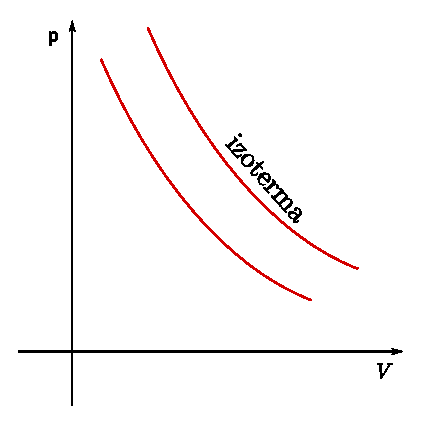
\includegraphics[width=\textwidth]{termo_4/termo_4_1}
            \newsubcap{Ideális gáznál az izotermák hiperbolák.}
            \label{fig:termo_4_1}
    \end{subfigure}\hfill
    \begin{subfigure}[t]{0.45\textwidth}
            \centering
            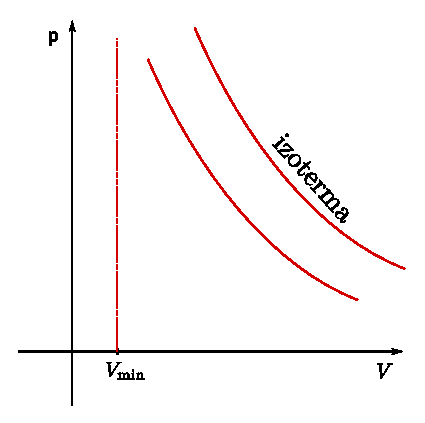
\includegraphics[width=\textwidth]{termo_4/termo_4_2}
            \newsubcap{Reális gázoknál van egy minimális térfogat, aminél kisebbre nem lehet összenyomni a gázt.}
            \label{fig:termo_4_2}
    \end{subfigure}
\end{figure}
Az ideális gáz állapotegyenlete emiatt már mindenképp javításra szorul:
\begin{align}\label{eq:vdW_1}
    \pres(V-nb) = nRT \follows \pres = \frac{nRT}{V-nb},
\end{align}
azonban nem vettük még figyelembe a kölcsönhatás járulékát. Mivel a van der Waals\footnote{\,Johannes Diderik van der Waals, 1837-1923.}-kölcsönhatás csak nagyon rövid távolságon taszító, egyébként pedig vonzó (de így is gyorsan lecsengő), ezért összességében kisebb nyomást fognak kifejteni a részecskék a doboz falának ütközve, ahogy ezt a \ref{fig:termo_4_3}. ábrán is szemléltetjük.
\begin{figure}
    \centering
    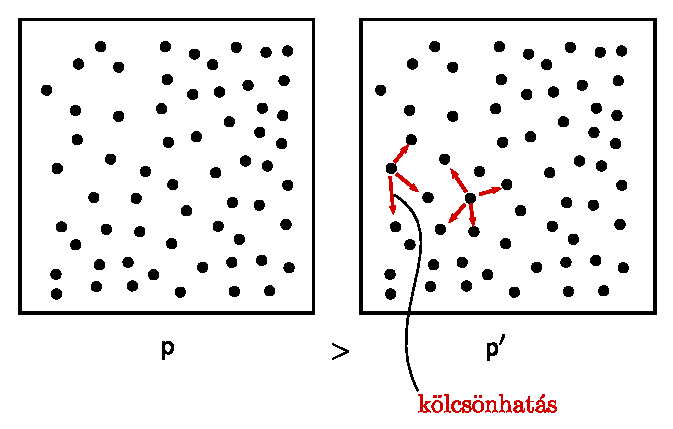
\includegraphics{termo_4/termo_4_3.eps}
    \caption{Van der Waals-gázoknál a nyomás csökken a részecskék vonzó kölcsönhatása miatt. Bal oldalon a kölcsönhatásmentes esetet látjuk, jobb oldalon pedig pár gázmolekulára berajzoltunk néhány rá ható erőt, ezt jelölik a piros nyilak.}
    \label{fig:termo_4_3}
\end{figure}
Igyekezzünk ezt megbecsülni! Ehhez tekintsünk egy egyszerűsített modellt, ahol a rövid távú kölcsönhatást egy konstans $-F_0$ erővel vesszük figyelembe $d$ távolságig (ld. \ref{fig:termo_4_5}. ábra), azaz:
\begin{align}
    F =
    \begin{cases}
    F_0<0,&\tn{ha}\quad r<d\\
    0,&\tn{egyébként}.
    \end{cases}
\end{align}
\begin{figure}[!h]
    \centering
    \begin{subfigure}[t]{0.45\textwidth}
            \centering
            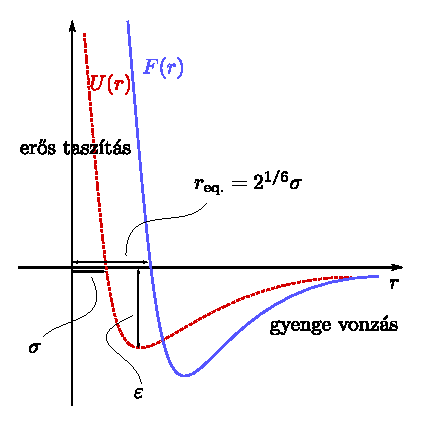
\includegraphics[width=\textwidth]{termo_4/termo_4_4}
            \newsubcap{Lennard--Jones-potenciál.}
            \label{fig:termo_4_4}
    \end{subfigure}\hfill
    \begin{subfigure}[t]{0.45\textwidth}
            \centering
            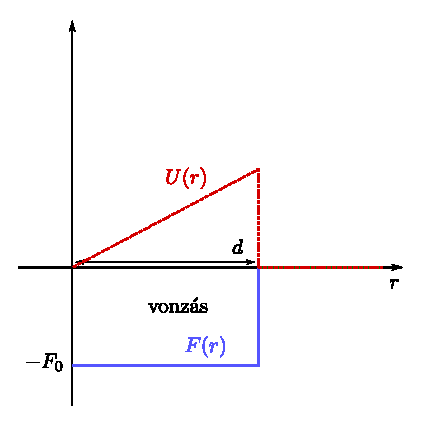
\includegraphics[width=\textwidth]{termo_4/termo_4_5}
            \newsubcap{A Lennard--Jones-potenciáls leegyszerűsített modellje konstans $-F_0$ erővel $d$ távolságig.}
            \label{fig:termo_4_5}
    \end{subfigure}
\end{figure}
Hogyan változik meg a nyomás ennek a kölcsönhatásnak a következtében? Egy gázrészecske annak $d$ sugarú környezetében $N_{\tn{pár}}$ számú részecskével hat kölcsön (ld. \ref{fig:termo_4_6}. ábra):
\begin{align}
    N_{\tn{pár}} \approx \overbrace{\rho\underbrace{Ad}_{=V}}^{\substack{\tn{részecskék}\\\tn{száma}}}\cdot\overbrace{\rho d^3}^{\substack{\tn{1 részecskére}\\\tn{jutó $d$}\\\tn{sugarú gömb}}},\quad \tn{ahol }\rho=\frac NV\tn{ a részecskesűrűség}.
\end{align}
\begin{figure}
    \centering
    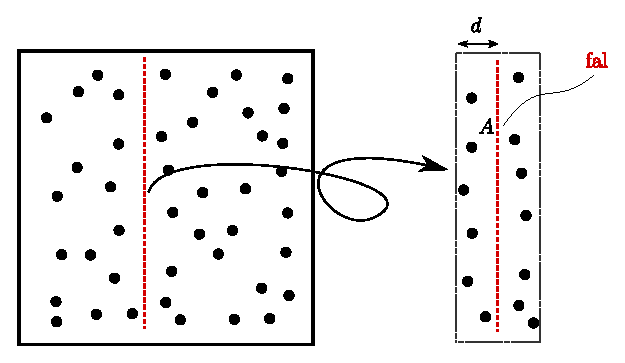
\includegraphics{termo_4/termo_4_6.eps}
    \caption{Rövid távú kölcsönhatás, mely a gázrészecskék $d$ sugarú környezetében hat.}
    \label{fig:termo_4_6}
\end{figure}
Ezekkel a teljes nyomás megváltozása:
\begin{align}
    \Delta\pres = \frac{F_{\tn{össz}}}{A}\sim \frac{F_0N_{\tn{pár}}}{A}\sim \frac{F_0}{A}\rho^2 A d^4 = F_0d^4\z{\frac nV}^2 = -a\z{\frac nV}^2,
\end{align}
ahol $a$ anyagi állandó, a negatív előjel pedig azért jelenik meg, mert a nyomás csökken a kölcsönhatásnak köszönhetően. A (\ref{eq:vdW_1}). egyenletet továbbírva kapjuk, hogy:
\begin{align}
    \pres = \frac{nRT}{V-nb}-a\z{\frac nV}^2 \follows \sz{\pres+a\z{\frac nV}^2}(V-nb) = nRT,
\end{align}
ez a \emph{van der Waals-gáz állapotegyenlete}, van der Waals érte Nobel-díjat kapott 1910-ben\footnote{\,Az állapotegyenlet kölcsönható rendszerek statisztikus fizikai számolásával is meghatározható, ugyanerre az eredményre jutunk elsőrendben.}. Az állapotegyenlet görbéi a $\pres-V$ síkon már nem hiperbolák, hanem bonyolult harmadfokú kifejezések. Kiszámolható az izoterm kompresszibilitás\footnote{\,Nem kell tudni, de $$\kappa_{vdW} = -\rec V \rec{\frac{2an^2}{V^3}-\frac{nRT}{(V-nb)^2}}$$.}, ami egy adott tartományon negatív is lehet, így ott a gáz instabillá válna, tehát ez egy tiltott tartomány, az izotermák (azonos hőmérsékletű görbe) ezt a tartományt ,,átugorják''. Keressük meg a kritikus pontot, ahol az $\pres-V$ grafikon egy izotermájának inflexiós pontja van, ahogy ez \aref{fig:termo_4_7}. ábrán is látható.
\begin{figure}
    \centering
    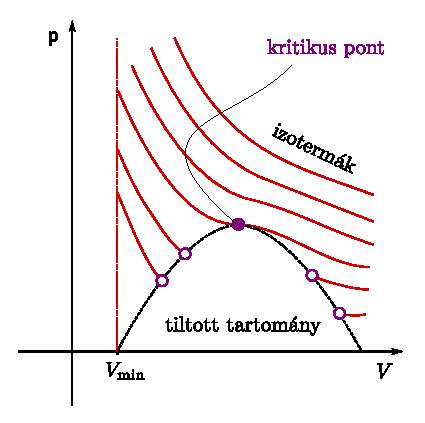
\includegraphics{termo_4/termo_4_7.eps}
    \caption{Van der Waals-gáz a $\pres-V$ diagramon. Látható rajta a kritikus pont, illetve a tiltott tartomány.}
    \label{fig:termo_4_7}
\end{figure}
A kritikus pont alatt a nyomásnak ugrása van, ami másodrendű (folytonos) fázisátalakulást jelent (a fáziátalakulásokról még részletesen szó fog esni a kurzus hátralévő részén). A kritikus pont értékeire adódik\footnote{\,Egyrészt a kompresszibilitás feltételéből adódik (ami ekvivalens a $\pd \pres V\big|_{T=T_c}=0$ feltétellel; itt $T_c$ a kritikus pont hőmérséklete): $$ \frac{2an^2}{V_c^3}-\frac{nRT_c}{(V_c-nb)^2}=0,$$
másrészt a $$\frac{\partial^2\pres}{\partial V^2}\bigg|_{T=T_c}=0$$ feltételből kapjuk, hogy:
$$\frac{2nRT_c}{(V_c-bn)^3}-\frac{6an^2}{V_c^4}=0.$$ Ebből a két egyenletből a kritikus pont paraméterei meghatározhatóak.}, hogy:
\begin{align}
    V_c = 3bn,\quad p_c = \frac{8}{27}\frac{a}{Rb},\quad T_c = \frac{1}{27}\frac{a}{b^2}.
\end{align}
\Aref{tab:vdW}. táblázatban felsoroltunk néhány tipikus értéket az anyagi állandókra és a kritikus értékekre:
\begin{table}[h!]
\centering
\begin{tabular}{|c|c|c|c|c|} \hline
Gáz & $a$ [$l^2\cdot$bar/mol$^2$] & $b$ [$l$/mol] & $T_c$ [K] & $p_c$ [bar]\\ \hline\hline
He & 0{,}0346 & 0{,}0238 & 5{,}18 & 2{,}26\\ \hline
O$_2$ & 1{,}382 & 0{,}0319 & 154{,}66 & 50{,}42\\ \hline
N$_2$ & 1{,}370 & 0{,}0387 & 126{,}22 & 33{,}88\\ \hline
CO$_2$ & 3{,}640 & 0{,}0427 & 303{,}95 & 73{,}94 \\ \hline
aceton & 16{,}02 & 0{,}112 & 510{,}00 & 47{,}30\\ \hline
\end{tabular}
\caption{A van der Waals-gáz anyagi állandói és kritikus pontjához tartozó értékek néhány minta esetén.}
\label{tab:vdW}
\end{table}